%Tema para beamer "CCM3" versión 1
%Desarrollo por Erick David Luna Núñez y 
%Fernanda Barajas Hernandez

\documentclass{beamer}

\usepackage[utf8]{inputenc}
\usepackage{xeCJK}
\usepackage{heuristica}
\usepackage[T1]{fontenc}
\usepackage[heuristica,vvarbb,bigdelims]{newtxmath}
\renewcommand*\oldstylenums[1]{\textosf{#1}}
\usepackage[sfdefault,scaled=.85]{FiraSans}
\usepackage{graphicx}
\usepackage[spanish]{babel} 
\usepackage[pages=some]{background}
\pagenumbering{arabic}



%%Se define el "environment" teorema
\newtheorem{teorema}{Teorema}

%Definir el autor con el estilo definido (el textbf y el uso del color son herramientas del diseño, no necesario borrar)
\title{\textbf{編譯器期末專題}}

%Nombre del autor
\author{
    李智修 / 張聯榮 / 林佑軒
} 

%Fecha o evento en que se presentará la plática
\date{報告日期: XXXX/XX/XX} 


%%Tema de beamer "CCM-3"
\usetheme{ccm3}

\begin{document}
%Define el fondo de la primer diapositiva
{\setbeamertemplate{background}{

\includegraphics[width=\the\paperwidth,height=\the\paperheight]{images/P3.png}}
%lo anterior es para definir el fondo de la primer diapositiva

\begin{frame}
  \titlepage %Necesario para generar la portada
\end{frame}

} %aquí termina el cambio de fondo

\begin{frame}
\tableofcontents %Imprime la tabla de contenido
\end{frame}

\section{使用環境及工具} %%Título de la sección (Opcional)
\subsection{環境}
\begin{frame}
  \frametitle{使用環境}
  \begin{itemize}
    \item 作業系統: Arch Linux %%[\checkmark] muestra una palomita al inicio de la línea
    \item 系統架構: x86\_64
    \item 
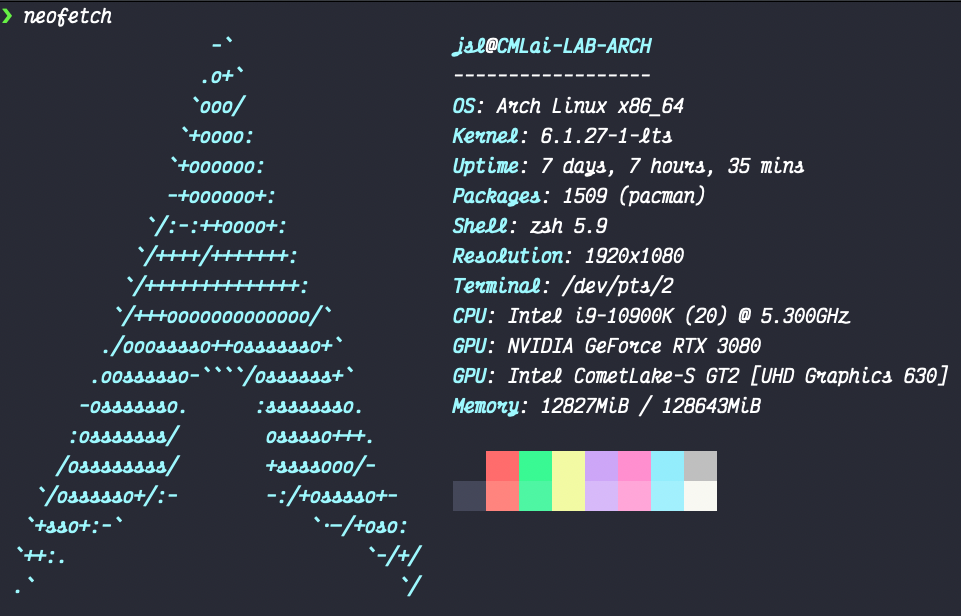
\includegraphics[width=260,height=160]{images/OS_INFO.png}
  \end{itemize}
\end{frame}

\subsection{工具}
\begin{frame}
  \frametitle{使用工具}
  \begin{itemize}
    \item Makefile: 自動化固定的步驟。
    \item flex, yacc: 將提供的.y, .l檔轉成自制的編譯器。
    \item clang, LLVM: 將程式轉成組合語言,然後編譯成可執行檔。
  \end{itemize}
\end{frame}

\section{實作過程}
\subsection{使用flex, yacc生出編譯器}
\begin{frame}{使用flex, yacc生出編譯器}
\begin{itemize}
    \item 我們首先參考了巴哈上的教學\cite{Lex},然後從這兩個地方\cite{ANSILex} \cite{ANSIYacc}取得了yacc, lex檔案。
    \item 然而我們發現無法直接使用指令編譯出檔案,因此我們又參考了Github上的討論串\cite{C99Grammars},得知了我們應該使用yacc -d的參數來編譯,而不是直接執行yacc: 
    \item 在同一個討論串中,我們也發現了yacc.y的檔案中需要再增加一個driver的函式(見下頁圖),否則會無法進行編譯。
    \item 其它的都很順例,就照步驟直接做就好了。
\end{itemize}
\end{frame}

\begin{frame}{使用flex, yacc生出編譯器}[fragile]
    圖在這裡。 yacc.y的最後一個函式(有driver註解地方的)
\end{frame}

\subsection{使用LLVM, clang生出組語、執行檔}
\begin{frame}
    \frametitle{使用LLVM, clang生出組語、執行檔}
\end{frame}

\section{Makefile實作}
\begin{frame}{使用Makefile加速測試過程}

\end{frame}

\section{參考資料}
\begin{frame}{參考資料}
    %posibles estilos para bibliografía: unsrt , siam , plain , ieeetr , alpha , acm , abbrv
    \bibliographystyle{abbrv}
  \bibliography{references}
\end{frame}

\section{Erwischt.}
\begin{frame}{以上,謝謝大家。}
    
\end{frame}

\end{document}